\documentclass[11pt]{beamer}
\usetheme{metropolis}
\usepackage[utf8]{inputenc}
\usepackage[english]{babel}
\usepackage[T1]{fontenc}
\usepackage{amsmath}
\usepackage{amsfonts}
\usepackage{amssymb}
\usepackage{bm}
\usepackage{subfig}
\usepackage{pgfplots}
\pgfplotsset{compat=newest}
\usepackage{multimedia}
%\usepackage{booktabs}
\newcommand{\Ex}{\mathbb{E}}
\newcommand{\Var}{\mathbb{V}\mathrm{ar}}
\newcommand{\Prob}{\mathbb{P}}
\DeclareMathOperator*{\argmin}{arg\,min}
\DeclareMathOperator*{\argmax}{arg\,max}
\newcommand{\Cov}{\textsf{Cov}}
\newcommand{\tra}{\mathrm{tr}}
\newcommand{\yobs}{\bm{y}^{\mathrm{obs}}}
\newcommand{\kest}{\hat{\bm{k}}}
\usetikzlibrary{positioning}
\DeclareMathOperator*{\KL}{\textsf{KL}}
\graphicspath{{./Figures/}}

\definecolor{blkcol}{HTML}{E1E1EA}
\definecolor{blkcol2}{RGB}{209, 224, 224}

% \definecolor{BlueTOL}{HTML}{222255}
% \definecolor{BrownTOL}{HTML}{666633}
% \definecolor{GreenTOL}{HTML}{225522}
% \setbeamercolor{normal text}{fg=BlueTOL,bg=white}
% \setbeamercolor{alerted text}{fg=BrownTOL}
% \setbeamercolor{example text}{fg=GreenTOL}
\setbeamercolor{block title}{bg = blkcol}
\setbeamercolor{block body}{bg = blkcol!50}


\title{Parameter control in the presence of uncertainties}
\author{{\large Victor Trappler } \\ Supervisors: Élise Arnaud, Laurent Debreu, Arthur Vidard}
\institute{AIRSEA Research team (Inria)-- Laboratoire Jean Kuntzmann \\
 \begin{center}

\includegraphics[scale=0.20]{INRIA_SCIENTIFIQUE_UK_CMJN}

\includegraphics[scale=0.20]{ljk}
\end{center}
}

\date{\today}
\setcounter{tocdepth}{1}


\begin{document}
\frame{
  \maketitle
}

\section{Introduction}
\frame{
\frametitle{Bottom friction}
\begin{itemize}
\item The friction of the ocean bed has an influence on the water circulation
\item Depends on the type and/or characteristic length of the asperities 
\item Subgrid phenomenon
\end{itemize}
\begin{center}
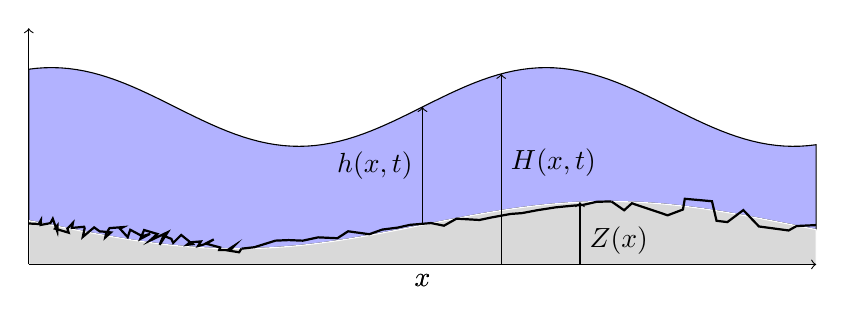
\begin{tikzpicture}
\usetikzlibrary{decorations.pathmorphing}

\definecolor{copper}{rgb}{0.69, 0.25, 0.21}
\definecolor{tin}{rgb}{0.7, 0.7, 0.7}

\tikzset{
  rugous1/.style = {black, thick,
    decoration={random steps,segment length=0.05cm,amplitude=.1cm}
  },
}
\tikzset{
  rugous2/.style = {black, thick,
    decoration={random steps,segment length=0.2cm,amplitude=.05cm}
  },
}
\tikzset{
  rugous3/.style = {black, thick,
    decoration={random steps,segment length=0.2cm,amplitude=.15cm}
  },
}

\filldraw [fill = blue!30]
   plot [samples = 100,domain = -5:5] (\x, {0.5*sin(\x r) + 2} )
-- plot [samples = 100,domain = 5:-5] (\x, {0.3*sin(\x/1.5 r)+0.5})
-- cycle;

\filldraw[fill = gray!30, draw = white]
   plot [samples = 100,domain = -5:5] (\x, {0.3*sin(\x/1.5 r)+0.5})
-- plot [samples = 100,domain = 5:-5] (\x, 0)
-- cycle;

\draw[rugous1, decorate](-5,0.52) -- (-2.3,0.2);
\draw[rugous2, decorate](-2.3,0.2) -- (2.4,0.8);
\draw[rugous3, decorate](2.4,0.8) -- (5,0.5);

\draw[->] (-5,0) -- (5,0);
\draw (0,0) node[below] {$x$};



\draw[->] (-5,0) -- (-5,3);

\draw[->] (0,0.5) -- (0,2);
\draw (0, 1.25) node[left] {$h(x,t)$} ;
\draw (0,0) node[below] {$x$};
\draw[->] (2,0) -- (2,{0.3*sin(2/1.5 r)+0.5});
\draw (2, 0.3) node[right] {$Z(x)$} ;
\draw[->] (1,0) -- (1,{0.5*sin(1 r)+2});
\draw (1, 1.3) node[right] {$H(x,t)$} ;
\end{tikzpicture}
\end{center}
}
% \frame{
%   \frametitle{Principles of Computer experiments}
%   \scalebox{0.7}{\input{../Figures/schema_bloc}}
% }

\frame{
\frametitle{Outline}
\tableofcontents
}
\section{Deterministic problem}
\frame[t]{
\frametitle{Computer code : the Shallow Water Equations}
\begin{itemize}
	\item[Input] 
	\begin{itemize}
		\item $\bm{k}$: Bottom friction (spatially distributed)
		\item $\bm{u}$: Environmental variables (fixed and known)
	\end{itemize}
	\item[Output] \begin{itemize}
	\item $W(\bm{k}) = \{W_i^n(\bm{k})\}_{i,n}$, where $W_i^n(\bm{k}) = [h_i^n(\bm{k}) \quad q_i^n(\bm{k})]^T$\\ for $0 \leq i \leq N_x$ and $0 \leq n \leq N_t$
	\end{itemize}
\end{itemize}
\vfill
\only<1>{\tikzstyle{block} = [rectangle, draw, fill=blue!20, 
     text centered, minimum width=1cm]

\tikzstyle{block2} = [rectangle, draw, fill=green!20, 
     text centered, rounded corners, minimum width=1cm]

\tikzstyle{LHS}=[rectangle, draw, text centered]

\begin{tikzpicture}[node distance=3cm]

\node [align = center] at (0,0) (input) {Control variable \\$K \in \mathcal{K}$};
%\node [align = center] at (4,1.5) (envir) {Environmental variables \\$\bm{u} \in \mathcal{U}$ fixed};
\node [align = center] at (4,1.5) (envir) {Environmental variables \\$\bm{x}_e \in \mathbb{X}$ fixed};

\node[block] at (4,0)(code){Direct Simulation};

\node[align = center] at (8,0) (output) {$W(K)$}; %\\ $\Rightarrow j(K)$};

\draw[->] (input) -- (code);
\draw[->] (envir) -- (code);
\draw[->] (code) -- (output);

\end{tikzpicture}}
\only<2>{\usetikzlibrary{positioning}
% \tikzstyle{block} = [rectangle, draw, fill=blue!30, 
%     text centered, minimum width=3em] 
 \tikzstyle{block} = [rectangle, draw, fill=blkcol, 
      text centered, minimum width=3em]

\tikzstyle{block2} = [rectangle, draw, fill=blkcol2, 
     text centered, rounded corners, minimum width=3em]

% \tikzstyle{block2} = [rectangle, draw, fill=blkcol2, 
%      text centered, rounded corners, minimum width=3em]

\tikzstyle{LHS}=[rectangle, draw, text centered]

\begin{tikzpicture}

%\node [align = center] at (0,0) (input) {Control variable \\$\mathbf{k} \in \mathbb{K}$};
\node [align = center] at (0,0) (input) {Control variable \\$\bm{k} \in \mathbb{K}$};
\node[block] at (4,0) (code){Direct Simulation};
%\node [align = center, above =of  code ] (envir) {Environmental variables \\$\mathbf{u} \in \mathbb{U}$ fixed};
\node [align = center] at (4,1.5) (envir) {Environmental variables \\$\bm{u} \in \mathbb{U}$ fixed};




%\node[align = center, right =of  code] (output) {$M(\mathbf{k})$};
\node[align = center] at (8,0) (output) {$\mathcal{M}(\bm{k},\bm{u})$};
%\node [align = center, right =of  inv, below = of output]  (obs) {$\mathbf{y}$};
\node [align = center] at (8,-1) (obs) {$\yobs$};
\node[block] at (4,-1) (inv) {Inverse Problem};

\draw[->] (input) -- (code);
\draw[->] (envir) -- (code);
\draw[->] (code) -- (output);

 % \node [align = center] at (0,0) (input) {$Y = \mathbb{H}M(K_{\mathrm{ref}})$};
 % \node [align = center] at (4,1.5) (envir) {Environmental variables \\$X_e$ r.v.};

 % \node[block] at (4,0)(code){"Inverse Problem"};

% \node[align = center] at (8,0) (output) {$K$};

\draw[->] (input) -- (code);
% \draw[->] (envir) -- (code);
\draw[->] (code) -- (output);
\draw[->] (output) -- (obs) ;
\draw[->] (inv) -|(input) ;
\draw[->] (obs) -- (inv);
\end{tikzpicture}}

}
\frame{
\frametitle{Data assimilation framework: Twin experiments}

Let us set $\bm{k}_{\mathrm{ref}}$\\
We have $\yobs = M(\bm{k}_{\mathrm{ref}}) = \{h_i^n(\bm{k}_{\mathrm{ref}})\}_{i,n}$ 
\begin{equation*}
j(\bm{k}) = \frac12 \|M(\bm{k}) - \bm{y}^{\mathrm{obs}} \|^2
\end{equation*} \pause
\begin{equation*}
\argmin_{\bm{k} \in \mathcal{K}}j(\bm{k}) ?
\end{equation*}


%\begin{itemize}
%\item<2-> Gradient-free: Simulated annealing, Nelder-mead,\dots
%$\rightarrow$ High number of runs, \alert<2>{very expensive}
%
%\item<3-> Gradient-based: gradient-descent, (quasi-) Newton method
%$\rightarrow$ Less number of runs, but \alert<3>{need the adjoint code}
%\end{itemize}
}
\section{Dealing with uncertainties}
\frame[t]{
\frametitle{Introducing the uncertainties}
Instead of considering $\bm{u}$ fixed, we consider that $\bm{U}$ is a random variable (pdf $\pi(\bm{u})$), and the output of the model depends on its realization. \\
\vfill
\only<1>{\usetikzlibrary{positioning}
% \tikzstyle{block} = [rectangle, draw, fill=blue!30, 
%     text centered, minimum width=3em] 
 \tikzstyle{block} = [rectangle, draw, fill=blkcol, 
      text centered, minimum width=3em]

\tikzstyle{block2} = [rectangle, draw, fill=blkcol2, 
     text centered, rounded corners, minimum width=3em]

% \tikzstyle{block2} = [rectangle, draw, fill=blkcol2, 
%      text centered, rounded corners, minimum width=3em]

\tikzstyle{LHS}=[rectangle, draw, text centered]

\begin{tikzpicture}

%\node [align = center] at (0,0) (input) {Control variable \\$\mathbf{k} \in \mathbb{K}$};
\node [align = center] at (0,0) (input) {Control variable \\$\bm{k} \in \mathbb{K}$};
\node[block] at (4,0) (code){Direct Simulation};
%\node [align = center, above =of  code ] (envir) {Environmental variables \\$\mathbf{u} \in \mathbb{U}$ fixed};
\node [align = center] at (4,1.5) (envir) {Environmental variables \\$\bm{u} \in \mathbb{U}$ fixed};




%\node[align = center, right =of  code] (output) {$M(\mathbf{k})$};
\node[align = center] at (8,0) (output) {$\mathcal{M}(\bm{k},\bm{u})$};
%\node [align = center, right =of  inv, below = of output]  (obs) {$\mathbf{y}$};
\node [align = center] at (8,-1) (obs) {$\yobs$};
\node[block] at (4,-1) (inv) {Inverse Problem};

\draw[->] (input) -- (code);
\draw[->] (envir) -- (code);
\draw[->] (code) -- (output);

 % \node [align = center] at (0,0) (input) {$Y = \mathbb{H}M(K_{\mathrm{ref}})$};
 % \node [align = center] at (4,1.5) (envir) {Environmental variables \\$X_e$ r.v.};

 % \node[block] at (4,0)(code){"Inverse Problem"};

% \node[align = center] at (8,0) (output) {$K$};

\draw[->] (input) -- (code);
% \draw[->] (envir) -- (code);
\draw[->] (code) -- (output);
\draw[->] (output) -- (obs) ;
\draw[->] (inv) -|(input) ;
\draw[->] (obs) -- (inv);
\end{tikzpicture}}
\only<2>{
\tikzstyle{block} = [rectangle, draw, fill=blkcol, 
     text centered, minimum width=1cm]
\tikzstyle{block2} = [rectangle, draw, fill=blkcol2, 
     text centered, rounded corners, minimum width=1cm]

\tikzstyle{LHS}=[rectangle, draw, text centered]

\begin{tikzpicture}[node distance=3cm]

\node [align = center] at (0,0) (input) {Control variable \\$\bm{k} \in \mathcal{K}$};
\node [align = center] at (4,1.5) (envir) {Environmental variables \\\alert<2>{$\bm{U}$ random}};
\node[block] at (4,0)(code){Direct Simulation};
\node[align = center] at (8,0) (output) {$W(\alert<2>{\bm{U}},\bm{k})$};
\node [align = center] at (8,-1) (obs) {$\yobs$};
\node[block] at (4,-1) (inv) {Inverse Problem};
\draw[->] (input) -- (code);
\draw[->] (envir) -- (code);
\draw[->] (code) -- (output);
\draw[->] (inv) -|(input) ;
\draw[->] (obs) -- (inv);
\draw[->] (output) -- (obs);
\end{tikzpicture}}
\vfill
}
\frame{
\frametitle{The cost function as a random variable}
\begin{itemize}
\item Output of the computer code ($\bm{u}$ is an input):
\begin{equation*}
    M(\bm{k}) \quad \text{becomes} \quad M(\bm{k},\bm{u})
\end{equation*}
\item The (deterministic) quadratic error is now
\begin{equation*}   
   j(\bm{k},\bm{u}) =  \frac12\|M(\bm{k},\bm{u}) - \yobs\|^2
\end{equation*}
\end{itemize}


%and for a given $K\in \mathcal{K}$, $j(\bm{X}_e,K)$ is a random variable
What to do with $j(\bm{k},\bm{U})$ (random variable) ?
}
\frame{
\frametitle{Variational approach or Bayesian approach ?}
\begin{itemize}
\item<1-> \textbf{Variational}: Minimize a function of $j(\bm{k},\bm{U})$, \\ e.g. Minimize $\Ex[j(\bm{K},\bm{U})|\bm{K} = \bm{k}]$.
\\ $\longrightarrow$ Precise objective
\item<2-> \textbf{Bayesian}: let us assume $e^{-j(\bm{k},\bm{u})} \propto p(\yobs|\bm{k},\bm{u})$  \\ Work around the likelihood and posterior distributions $p(\bm{k}|\yobs)$  \\
$\longrightarrow$ More general method
\end{itemize}
\onslide<3-> But
\begin{itemize}
\item Dependent on the efficiency of the statistical estimators
\item Knowledge of $\bm{U}$ ? Assumptions on error ?
\item Computational cost ?
\end{itemize}
}
%\frame{
%\frametitle{Issues raised}
%%Random variable : $J(\bm{X}_e,K)$
%\begin{tabular}{ll}
%Influence of $\bm{X}_e$ ? & \onslide<2->{ $\longrightarrow$ Sensitivity analysis}\\
%Computational cost ? & \onslide<2->{ $\longrightarrow$ Use of surrogate}
%\end{tabular}
%}


\section{Robust minimization}

\subsection{Concepts of robustness}
\frame{
	\frametitle{An illustration}
	$(\bm{u},\bm{k}) \mapsto f(\bm{u},\bm{k}) = \tilde{f}(\bm{u}+\bm{k})$ \\ $\bm{U} \sim \mathcal{N}(0,s^2)$ truncated on $[{-3};3]$. Plot of $f(0,\cdot) = \tilde{f}(\cdot)$ \vfill
	\begin{figure}[!h]
	\centering
	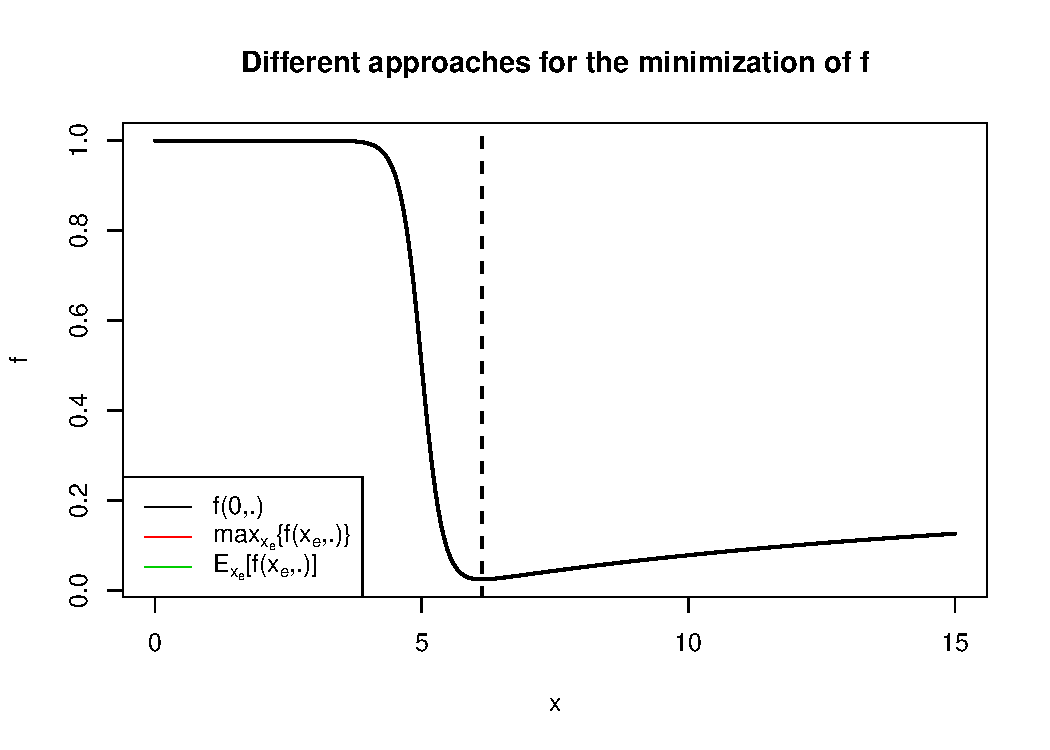
\includegraphics[scale = 0.5]{./Figures/mean_worstcase_robustness1}
	\end{figure}
}
\frame{
	\frametitle{An illustration}
	$(\bm{u},\bm{k}) \mapsto f(\bm{u},\bm{k}) = \tilde{f}(\bm{u}+\bm{k})$ \\ $\bm{U} \sim \mathcal{N}(0,s^2)$ truncated on $[{-3};3]$. {\color{red}	Plot of $\max_{\bm{u}} \{f(\bm{u},\cdot)\}$} \vfill
	\begin{figure}[!h]
	\centering
	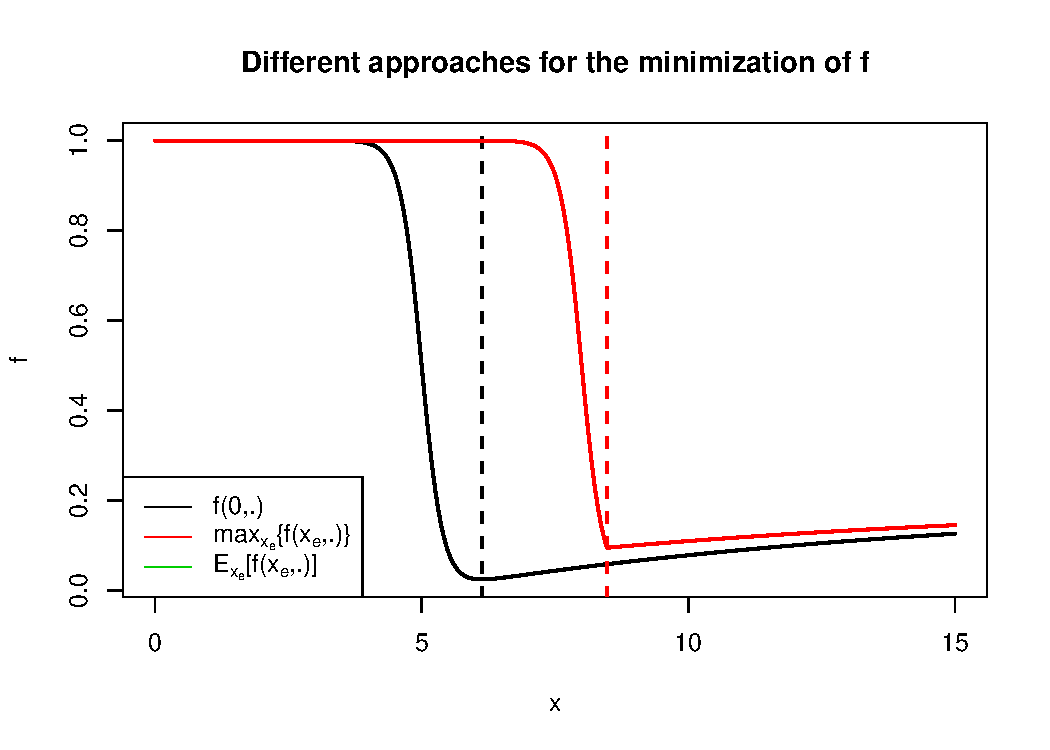
\includegraphics[scale = 0.5]{./Figures/mean_worstcase_robustness2}
	\end{figure}
}
\frame{
	\frametitle{An illustration}
	$(\bm{u},\bm{k}) \mapsto f(\bm{u},\bm{k}) = \tilde{f}(\bm{u}+\bm{k})$ \\ $\bm{U} \sim \mathcal{N}(0,s^2)$ truncated on $[{-3};3]$. {\color{green} Plot of $\Ex_{\bm{u}}[f(\bm{u},\cdot)]$} \vfill
	\begin{figure}[!h]
	\centering
	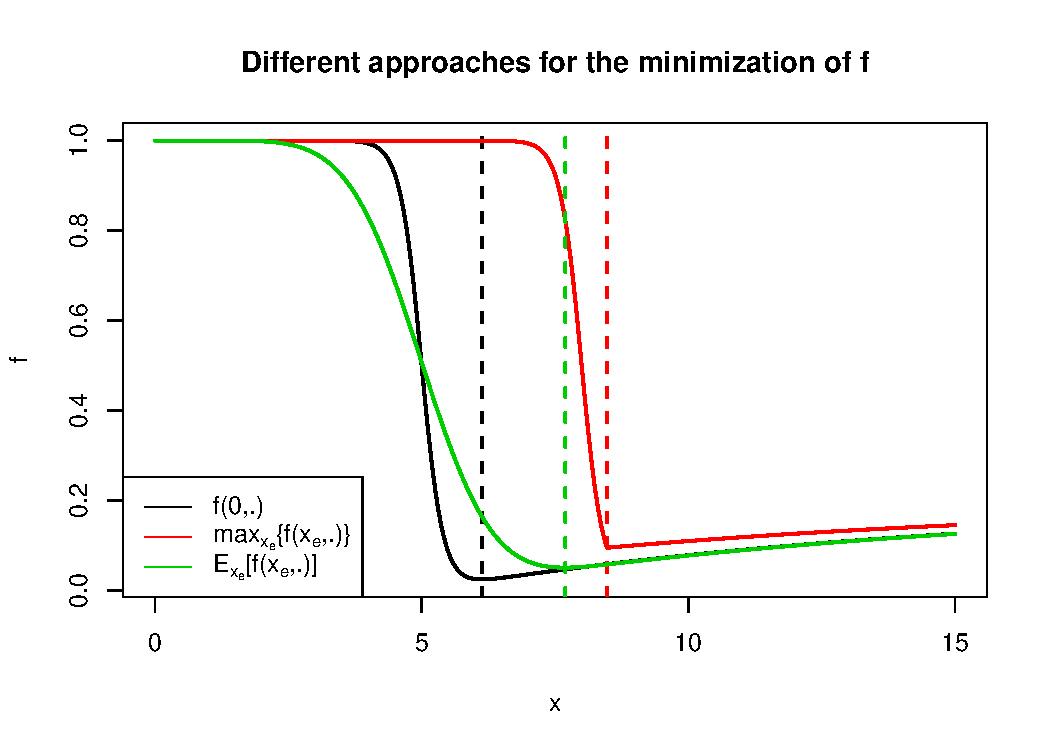
\includegraphics[scale = 0.5]{./Figures/mean_worstcase_robustness3}
	\end{figure}
}
\frame{
  \frametitle{Variational Approach}
  \textbf{Non-exhaustive list of ``Robust'' Objectives }
\begin{itemize}
\item Global Optimum: $ \min_{(\bm{k},\bm{u})} j(\bm{u},\bm{k})$ $ \longrightarrow $ EGO
\item Worst case: $ \min_{\bm{k}} \max_{\bm{u}} j(\bm{u},\bm{k})$ $ \longrightarrow $ Explorative EGO
\item M-robustness: $\min_{\bm{k}} \Ex\left[j(\bm{U},\bm{k})\right] \longrightarrow $ iterated LHS
\item V-robustness: $\min_{\bm{k}} \Var\left[j(\bm{U},\bm{k})\right] \longrightarrow $ gradient-descent with PCE
\item $\rho$-robustness: $\min \rho(j(\bm{U},\bm{k}))$ $\longrightarrow$ gradient-descent with PCE
\item Multiobjective: choice within Pareto frontier $\longrightarrow$ 1L/2L kriging
\end{itemize}

}


\subsection{Bayesian inference}
\frame{
  \frametitle{Bayesian approach}
  Let us suppose $\bm{K} \sim \pi(\bm{k})$.
  
  Having observed $\yobs$, joint distribution of $(\bm{K},\bm{U})$: $p(\bm{k},\bm{u}|\yobs)$ ? 
\begin{block}{Bayes' Theorem}<2->
\begin{align*}
p(\bm{k},\bm{u} | \yobs) &\propto p(\yobs| \bm{k},\bm{u})\pi(\bm{k},\bm{u}) \\
					& \propto \alert{L(\bm{k},\bm{u}; \yobs)} \pi(\bm{k})\pi(\bm{u})
\end{align*}
\end{block}
\onslide<3->
Link with cost function $j$ : Squared error $\leftrightarrow$ Gaussian errors
\begin{align*}
  L(\bm{k},\bm{u}; \yobs) &\propto \exp\left[- \tfrac{1}{2}\|M(\bm{k},\bm{u}) - \yobs \|^2_{\bm{\Sigma}^{-1}} \right] = \exp\left[-j(\bm{k},\bm{u})\right]
\end{align*}
}
\frame{
  \frametitle{Bayesian Quantities of interest}
% \newline
  \begin{block}{Bayes' theorem}
    $p(\bm{k},\bm{u}|\yobs) \propto L(\bm{k},\bm{u}; \yobs) \pi(\bm{k})\pi(\bm{u})\propto \alert{p(\bm{k}|\yobs,\bm{u})}\pi(\bm{u})$
    \end{block}
    \begin{align*}
    \text{ML :}   & \quad\argmax_{(\bm{k},\bm{u})} L(\bm{k},\bm{u}; \yobs) \\
    \text{MAP :}  & \quad \argmax_{(\bm{k},\bm{u})} p(\bm{k},\bm{u}| \yobs)= L(\bm{k},\bm{u}; \yobs)\pi(\bm{k})\pi(\bm{u})\\
    \alert<2>{\text{MMAP :}} & \quad \argmax_{\bm{k}} p(\bm{k}|\yobs) = \int_{\mathcal{U}} p(\bm{k},\bm{u}| \yobs) \,\mathrm{d}\bm{u} \\
    \alert<2>{\text{Min of variance :}} & \quad \argmin_{\bm{k}} \Var_{U}\left[p(\bm{k}| \yobs, \bm{U})\right] \\
      \alert<2>{\text{Worst Case:}} & \quad \argmax_{\bm{k}} \{\min_{\bm{u}} p(\bm{k}|\yobs,\bm{u}) \} \\
          \alert<2>{\text{MPE :}} & \quad \text{Mode of } \bm{K}_{\argmax}= \argmax_{\bm{k}} p(\bm{k} | \yobs, \bm{U})
  \end{align*}
}
\frame{
  \frametitle{Illustration on the SWE}
  \begin{centering}
    Family of densities: $\{ p(\bm{k}|\yobs,\bm{u});\bm{u} \in \mathcal{U}\}$
    \end{centering}
\begin{columns}
  \begin{column}{0.38\linewidth}

    \emph{MMAP}:
     $ \argmax_{\bm{k}} p(\bm{k}|\yobs)$ \\
    \emph{Min Var}:
      $\argmin_{\bm{k}} \Var_{U}\left[p(\bm{k}| \yobs, \bm{U})\right]$ \\
    \emph{Worst case}:
      $\argmax_{\bm{k}} \{\min_{\bm{u}} p(\bm{k}|\yobs,\bm{u}) \}$ \\
\end{column}
\begin{column}{0.62\linewidth}
\begin{center}
 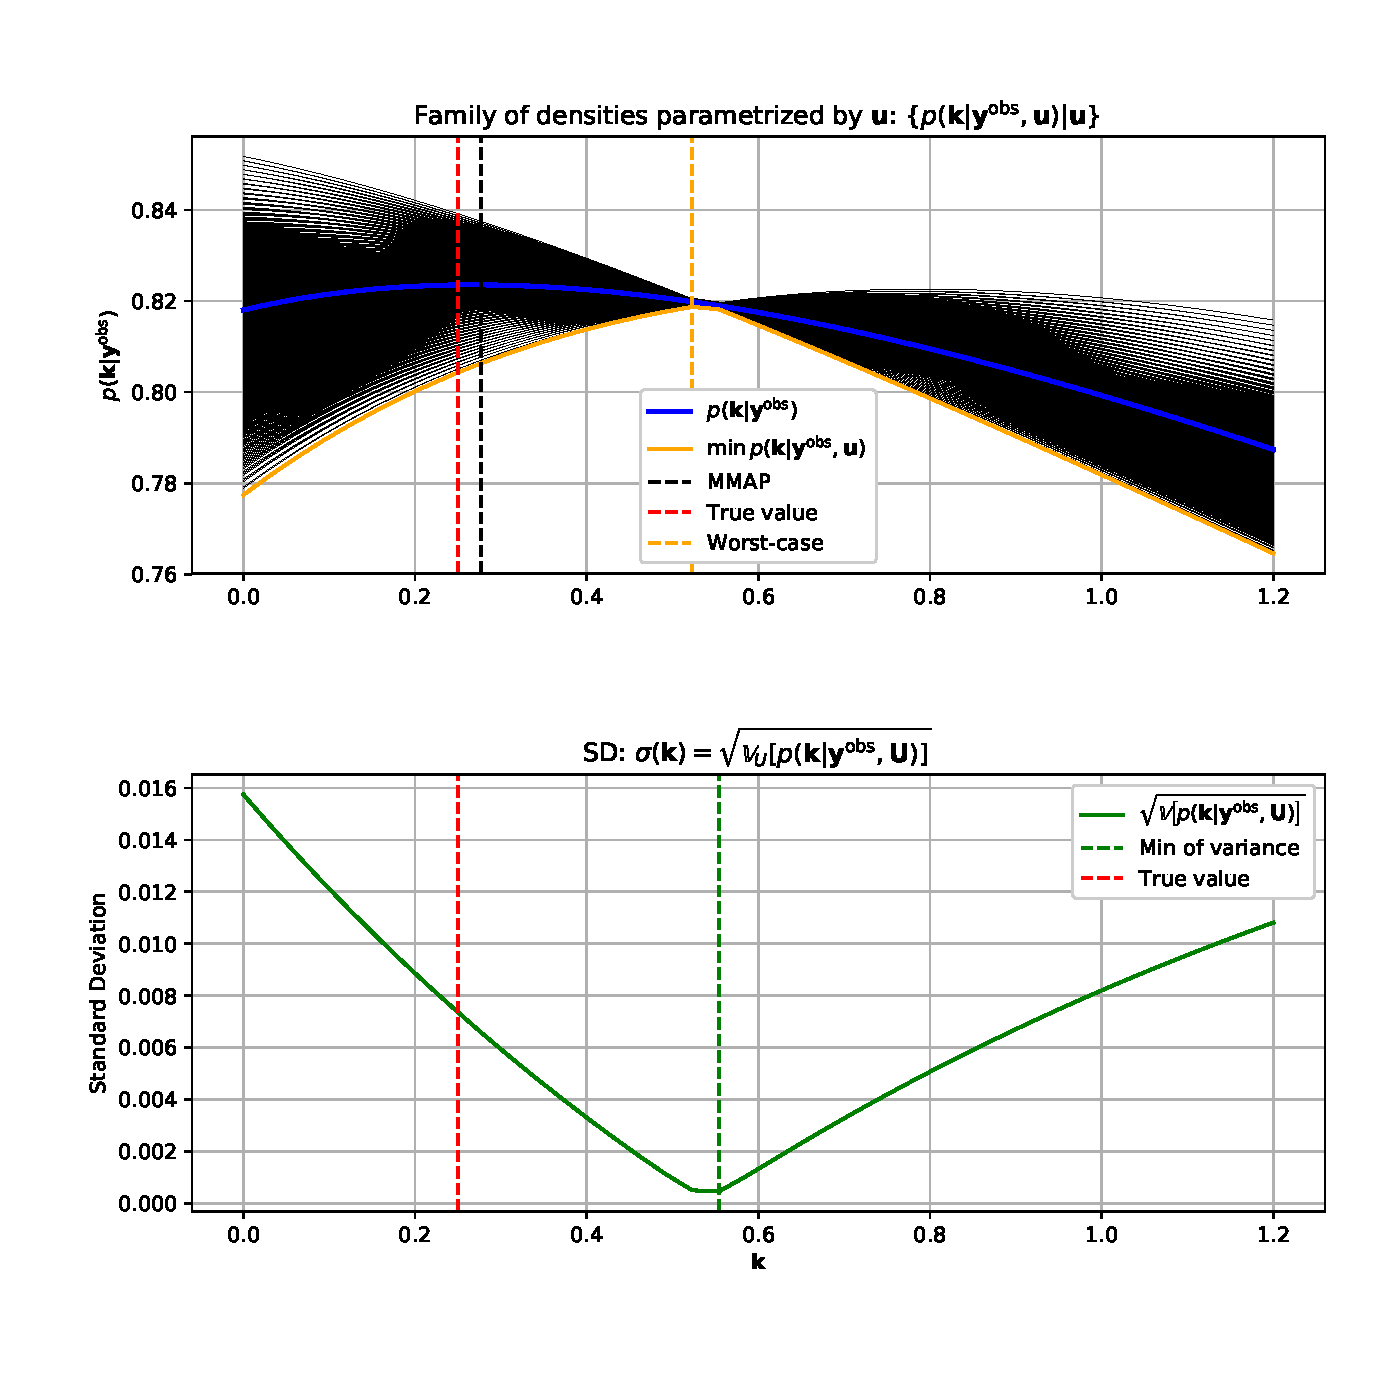
\includegraphics[width = \linewidth, height = .9\textheight]{MMAP_minvariance}
\end{center}
\end{column}
\end{columns}
}
\frame{
  \frametitle{``Most Probable Estimate''}
  $\bm{K}_{\argmax}= \argmax_{\bm{k}\in\mathcal{K}} p(\bm{k} | \yobs,\alert{\bm{U}})$ random variable \\
  $\longrightarrow$ estimate its density (how often is the value $\bm{k}$ a maximizer)

  Straightforward algorithm:
  \begin{itemize}
\item For $i=1\dots N$:
    \begin{itemize}
  \item Sample $\bm{u}^{(i)}$ from $\pi(\bm{u})$ / Adapted space-filling designs
  \item Maximize $p(\bm{k}|\yobs,\bm{u}^{(i)})$ yielding $\bm{k}_{\argmax}^{(i)}$ (adjoint method)
  \end{itemize}
  \item Estimate density (KDE) / Mode
  \end{itemize}
 }
\frame{
  \frametitle{Illustration of MPE}
  \movie[width = \linewidth, height= \textheight, poster, showcontrols]{}{animation.mpg}
}
\section{Surrogates and optimization}
\frame[t]{
\frametitle{Why surrogates?}
\begin{itemize}
\item Computer model: \alert{expensive to run}
\item $\dim \mathcal{K}$ , $\dim \mathcal{U}$ can be very large: \alert{curse of dimensionality}
\item Uncertainties upon $\bm{u}$ directly in the surrogate
\end{itemize}
\vfill
\begin{center}
	\only<1>{\scalebox{0.9}{
\tikzstyle{block} = [rectangle, draw, fill=blue!20, 
     text centered, minimum width=1cm]
\tikzstyle{block2} = [rectangle, draw, fill=green!20, 
     text centered, , minimum width=6cm]

\tikzstyle{LHS}=[rectangle, draw, text centered]

\begin{tikzpicture}[node distance=3cm]

\node [align = center] at (0,0) (input) {Control variable \\$K \in \mathcal{K}$};
\node [align = center] at (4,1.5) (envir) {Environmental variables \\$\bm{X}_e$ random};
\node[block] at (4,0)(code){Direct Simulation};
\node[align = center] at (7,0) (output) {$W(\bm{x}_e,K)$};
\node[align = center] at (9.2,0) (jfun) {$j(\bm{x}_e,K)$};
\draw[->] (input) -- (code);
\draw[->] (envir) -- (code);
\draw[->] (code) -- (output);
\draw[->] (output) --(jfun);



\end{tikzpicture}}}	
	\only<2>{\scalebox{0.9}{
\tikzstyle{block} = [rectangle, draw, fill=blue!20, 
     text centered, minimum width=1cm]
\tikzstyle{block2} = [rectangle, draw, fill=green!20, 
     text centered, , minimum width=6cm]

\tikzstyle{LHS}=[rectangle, draw, text centered]

\begin{tikzpicture}[node distance=3cm]

\node [align = center] at (0,0) (input) {Control variable \\$K \in \mathcal{K}$};
\node [align = center] at (4,1.5) (envir) {Environmental variables \\$\bm{X}_e$ random};
\node[block] at (4,0)(code){Computer Code};
\node[align = center] at (7,0) (output) {$W(\bm{x}_e,K)$};
\node[align = center] at (9.2,0) (jfun) {$\bar{j}(\bm{x}_e,K)$};
\draw[->] (input) -- (code);
\draw[->] (envir) -- (code);
\draw[->] (code) -- (output);
\draw[->] (output) --(jfun);
\node[block2] at (5,0) (surr) {Metamodel};
\draw[->] (input) -- (surr);


\end{tikzpicture}}}
\end{center}
\vfill
}
\frame{
\frametitle{Using surrogates for optimization : adaptative sampling}
Based on kriging model ( =Gaussian Process Regression) $\longrightarrow$ mean and variance \\
How to choose a new point to evaluate ? 
Criterion $\kappa(\bm{x}) \longrightarrow$ "potential" of the point
\begin{equation*}
\bm{x}_{\mathrm{new}} = \argmax \kappa(\bm{x})
\end{equation*}
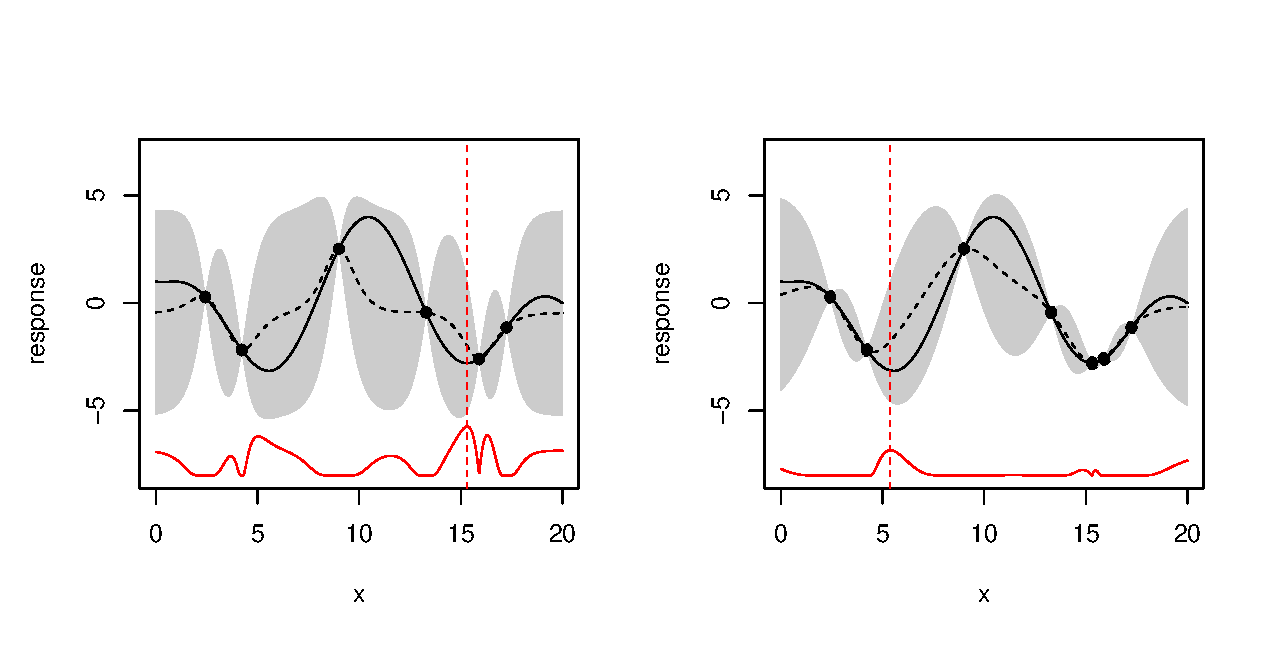
\includegraphics[width = \textwidth]{example_EGO}
}

\section{Conclusion}
\frame{
\frametitle{Conclusion}
\begin{block}{Wrapping up}
\begin{itemize}
\item Variational and bayesian approaches for this inverse problem results in different methods
\item In both case, strategies rely heavily on surrogate models $\longrightarrow$ Kriging, Polynomial chaos
\end{itemize}
\end{block}


\begin{block}{Perspective and future work}
\begin{itemize}
\item Cost of computer evaluations $\rightarrow$ limit the total number of runs
\item Dimensionality of the input space $\rightarrow$ reduction of the input space ?
\item How to deal with uncontrollable errors $\rightarrow$ errors between model and reality ?
\end{itemize}
\end{block}
}

\end{document}